%My Beamer Template for Surgery Presentations
%Prepared by Dr Suman (MS)

%Edit it and make your own

\documentclass[12pt]{beamer}
\usepackage[english]{babel}
%No need to include  graphicx, Beamer loads it itself.
\usetheme{AnnArbor}
\usecolortheme{beaver}
\setbeamertemplate{caption}[numbered]
\setbeamercolor{block title}{bg=green!70,fg=black}






\title[Presentation]{My Awesome Presentation\\on Surgery in Nepal}
\author[sumandoc]{Dr Suman\\
\small \texttt{suman\dots@gmail.com}}
\date{\today}
\institute[XY University]{\normalsize Institute of Medicine, XY University}



%begin document 

\begin{document}

%Title slide
\begin{frame}
\maketitle
\end{frame}


%section goes here. It appears in each slide in Warsaw and Berkeley theme. And they remain highlighted in the slides under those sections.
\section{Introduction}
\subsection{Discuss here}

%Other slide


\begin{frame}
I will show you to make presentation with \LaTeX and beamer. Bear with me.
\end{frame}
\begin{frame}{Slide 2}
\framesubtitle{This is subtitle}
\begin{itemize}
	\item Scalpel
	\item Cautery
	\item Suture 
\end{itemize}

\begin{block}{Monthly meet of SSN}
	It takes place every last Saturday of Nepali calendar.\\You are invited. {:)}
\end{block}
\end{frame}

\section{Section 2}

\begin{frame}{Slide 3}
	\begin{itemize}
		\item {Surgery is rewarding.}
		\item Mmm\dots\footnote{This is first footnote. You can cite journal here} 
		\item Neurosurgery Society\footnote{Journal of SSN}
	\end{itemize}
\end{frame}

\begin{frame}{Slide 4}
We are about to end this presentation.\footnote{This is second footnote. You can cite journal here also. :)}
\end{frame}

\begin{frame}{Inserting images}
Now I am including image in my presentation.
 
\begin{columns}
	\column[]{0.5\paperwidth}
	\begin{figure}
		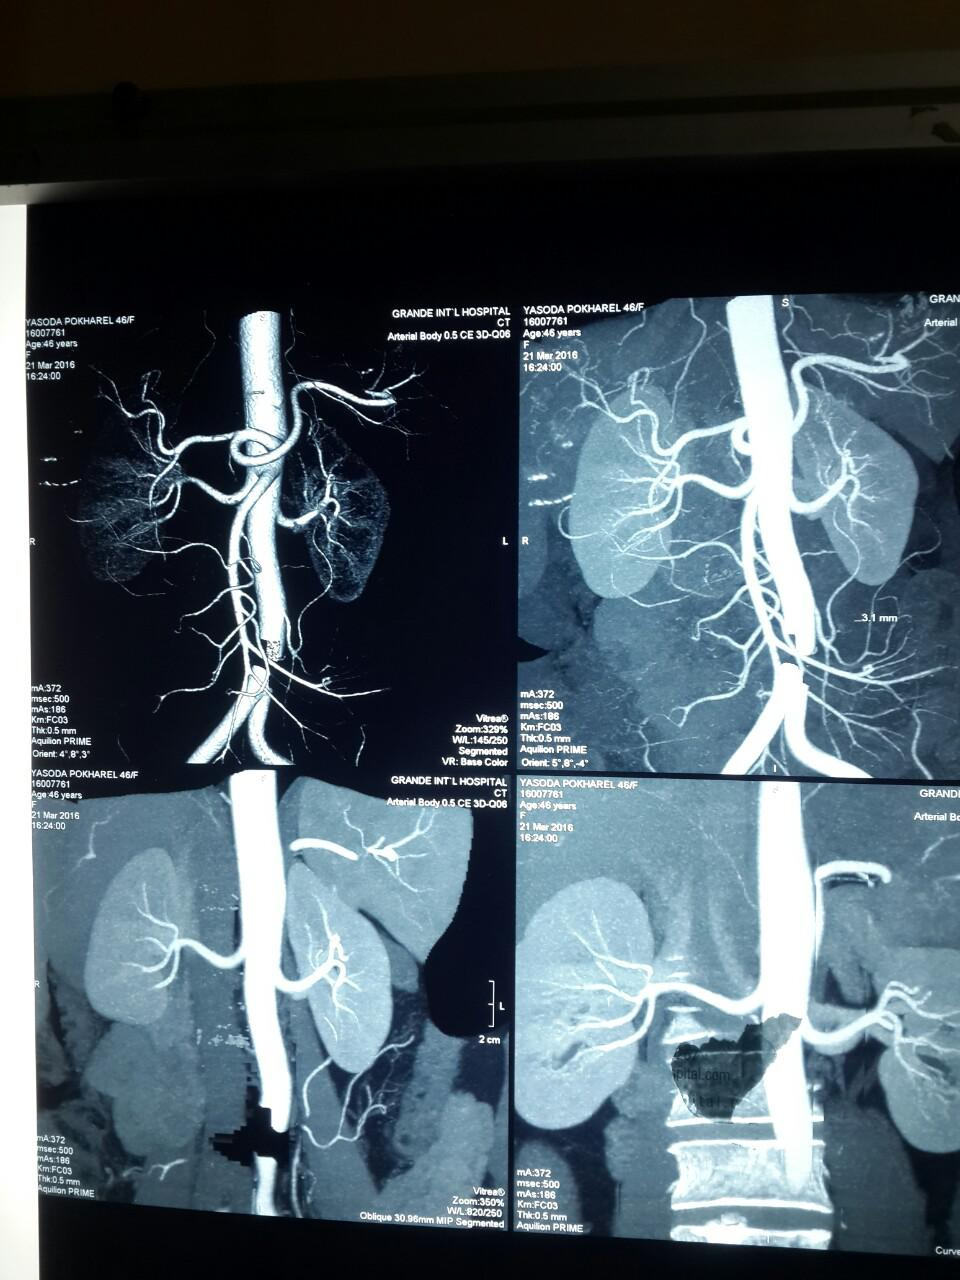
\includegraphics[height=50mm, width=50mm]{yasoda.jpg}
		\caption{CT angiography of a donor patient for renal transplantation.}
	\end{figure}
   \column[]{0.5\paperwidth}
   \begin{figure}
   	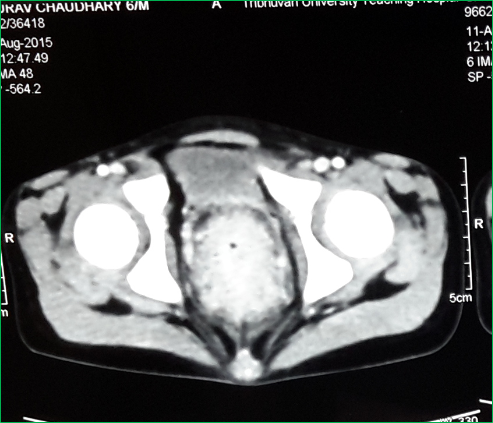
\includegraphics[height=50mm, width=50mm]{Picture1.png}
   	\caption{CT scan showing growth in rectum}
   \end{figure}
\end{columns}

\end{frame}

\begin{frame}{Repeat image}
\begin{figure}
	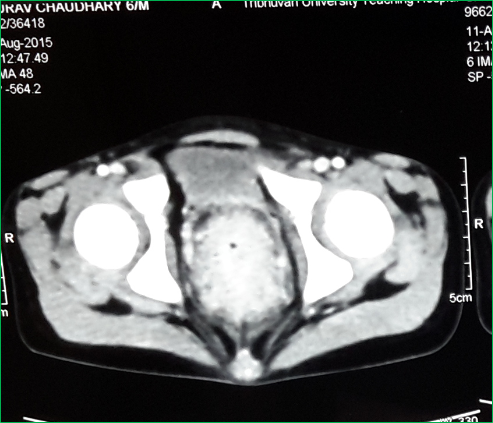
\includegraphics[height=65mm, width=80mm]{Picture1.png}
	\caption{CT scan showing growth in rectum}
\end{figure}
\end{frame}

\begin{frame}{Last slide}
	\centering \Huge Thank you for coming till here. See u next time. {:-)}	
\end{frame}
\end{document}